% =============================================================================
%  A Digital Twin-Based State Estimation Framework for Decision Support
%  in Primary Crushing Mining Operations
%
%  Proyecto de Investigacion (ACIF3002) - Universidad Andres Bello
%
%  Compilacion en Overleaf: pdfLaTeX + BibTeX
%    Menu -> Settings -> Compiler: pdfLaTeX
%  Secuencia local: pdflatex -> bibtex -> pdflatex -> pdflatex
% =============================================================================

\documentclass[conference]{IEEEtran}
\IEEEoverridecommandlockouts

\usepackage{cite}
\usepackage{amsmath,amssymb,amsfonts}
\usepackage{algorithmic}
\usepackage{graphicx}
\usepackage{textcomp}
\usepackage{xcolor}
\usepackage{booktabs}
\usepackage[T1]{fontenc}
\usepackage[utf8]{inputenc}
\usepackage{url}

\def\BibTeX{{\rm B\kern-.05em{\sc i\kern-.025em b}\kern-.08em
    T\kern-.1667em\lower.7ex\hbox{E}\kern-.125emX}}

\begin{document}

\title{A Digital Twin-Based State Estimation Framework\\
for Decision Support in Primary Crushing Mining Operations}

\author{
\IEEEauthorblockN{Daniel A. Prado Correa}
\IEEEauthorblockA{\textit{Facultad de Ingenier\'ia} \\
\textit{Universidad Andr\'es Bello}\\
Santiago, Chile}
\and
\IEEEauthorblockN{Omar I. Salinas Silva}
\IEEEauthorblockA{\textit{Facultad de Ingenier\'ia} \\
\textit{Universidad Andr\'es Bello}\\
Santiago, Chile}
\and
\IEEEauthorblockN{Jorge I. V\'asquez}
\IEEEauthorblockA{\textit{Facultad de Ingenier\'ia y Ciencias} \\
\textit{Universidad Adolfo Ib\'a\~nez}\\
Santiago, Chile}
}

\maketitle

% =============================================================================
\begin{abstract}
Modern mining operations increasingly rely on digital twins to support
operational decision-making, yet most proposed architectures implicitly assume
that the sensor and SCADA data feeding them are clean and complete. In primary
crushing stations this assumption fails: severe mechanical vibration and
abrasive airborne dust degrade level telemetry, and operationally relevant
variables such as the instantaneous discharge rate of the crusher are not
instrumented at all. This paper proposes and validates a decoupled analytical
software module that acts as a physical-consistency layer between degraded
telemetry and the decision layer of a mining digital twin. The module couples a
mass-conservation state-space model of the crusher feed hopper with a discrete
linear Kalman filter, and is validated through Monte Carlo simulation with a
fixed pseudorandom seed. Over $M=50$ independent runs of $N=1000$ steps, the
module reduces the mean squared error of the retained volume by 89.57\,\% with
respect to the raw SCADA baseline, a reduction that is statistically significant
under a paired $t$-test and confirmed by a Wilcoxon signed-rank test after the
normality assumption is empirically rejected. More notably, for the unsensed
filling rate the module reduces the error by 98.17\,\% relative to finite
differencing of the raw signal, which indicates that the analytical layer does
not merely denoise available data but generates observability where
instrumentation provides none. A covariance mismatch analysis shows that
performance is governed by the $\mathbf{Q}/\mathbf{R}$ ratio rather than by
absolute values, which substantially lowers the practical tuning barrier for
industrial adoption.
\end{abstract}

\begin{IEEEkeywords}
digital twin, state estimation, Kalman filter, partial observability, mining
operations, decision support, cyber-physical systems, SCADA
\end{IEEEkeywords}

% =============================================================================
\section{Introduction}

The mining sector is undergoing a rapid digital transformation driven by the
need to improve productivity, safety, energy efficiency and operational
resilience. In this context, digital twins, industrial simulation and artificial
intelligence have emerged as promising tools for supporting operational
decision-making \cite{fuller2020,liu2021,qu2023}.

However, many AI- and simulation-driven systems assume that the operational
state of the process is fully known. In practice, mining systems are only
partially observable: measurements are noisy, delayed or incomplete, and several
variables of interest are not directly sensed. This creates a gap between the
physical layer and the digital decision layer.

Primary crushing is the foundational link of the copper comminution chain and
illustrates the problem sharply. Extraction trucks discharge ore
discontinuously into a feed hopper while the crusher extracts material
continuously. The retained volume governs process continuity: too low a level
produces idle operation and energy inefficiency, while too high a level leads to
blockages and unscheduled downtime. Supervision relies on ultrasonic level
transducers whose signals are degraded by the continuous mechanical vibration
and the high concentration of abrasive dust characteristic of the crushing
station. The instantaneous extraction rate, which varies with ore hardness, has
no direct instrumentation at all.

Traditional automation processes this raw telemetry using deterministic
algorithms or fixed-threshold alarms, which fail to capture stochastic process
disturbances. When corrupted SCADA data are fed directly into higher-level
optimization tools, automated decision-making degrades into suboptimal control
strategies. This work addresses that analytical gap by designing a decoupled
software module that performs recursive state estimation and delivers a
physically consistent state to the digital twin.

The contribution of this work is threefold:

\begin{enumerate}
\item a dynamic-systems formulation of the primary crushing feed hopper suitable
      for digital twin development, in which the unsensed extraction rate is
      modeled as a latent state and formal observability is established;
\item a decoupled state estimation layer that fuses SCADA observations with the
      mass-conservation process model, validated by Monte Carlo simulation with
      formal hypothesis testing and an explicit verification of its
      distributional assumptions; and
\item a quantitative characterization of the module's robustness to sensor
      degradation and to covariance mistuning, which establishes the operating
      envelope within which the module remains useful.
\end{enumerate}

The remainder of the paper is organized as follows. Section~\ref{sec:related}
reviews related work. Section~\ref{sec:problem} formulates the problem.
Section~\ref{sec:method} describes the methodology. Section~\ref{sec:results}
reports the results, Section~\ref{sec:discussion} discusses them, and
Section~\ref{sec:conclusion} concludes.

% =============================================================================
\section{Related Work}
\label{sec:related}

\subsection{Digital Twins and Cyber-Physical Systems}

The cyber-physical systems paradigm was formulated by Lee \cite{lee2008} as the
tight integration of computational and physical processes, noting that the
central challenge is the fidelity of the coupling rather than computation
itself. Uhlemann \textit{et al.} \cite{uhlemann2017} proposed the digital twin
as a concrete realization of the cyber-physical production system for Industry
4.0, and Tao \textit{et al.} \cite{tao2019} oriented it towards prognostics and
health management of complex equipment. Fuller \textit{et al.}
\cite{fuller2020} systematized enabling technologies and open challenges, and
Liu \textit{et al.} \cite{liu2021} consolidated a review of concepts,
technologies and industrial applications.

A shared omission emerges from these works: all of them tacitly assume a
sufficiently clean telemetry network. Uhlemann \textit{et al.}
\cite{uhlemann2017} locate the data gap at the middleware and interoperability
layer, while \cite{tao2019} and \cite{fuller2020} focus on architecture and
synchronization rather than on input signal fidelity. Sepasgozar
\cite{sepasgozar2021} names this tension most precisely by distinguishing the
\textit{digital shadow}, which mirrors raw data, from the \textit{digital twin}
proper, which processes and removes the underlying uncertainty. This
distinction is adopted here as a design criterion: without an explicit
mathematical denoising layer, what is built is not a digital twin but a
high-resolution digital shadow.

\subsection{Digital Twins in the Minerals Industry}

Qu \textit{et al.} \cite{qu2023} provide a comprehensive review of digital twins
in the minerals industry and report growing but fragmented adoption,
concentrated in planning and haulage rather than in comminution stages. The more
recent systematic review by Ebad \textit{et al.} \cite{ebad2026}, covering 68
studies published between 2015 and 2025 on AI-driven digital twins in mining,
reports a marked predominance of machine learning and deep learning methods and
identifies data integration, real-time processing and limited industrial
validation as persistent challenges.

Read jointly, both reviews support a relevant observation: research effort in
mining digital twins has concentrated on the upper learning and prediction
layers, while the intermediate physical-consistency layer remains comparatively
unattended.

\subsection{State Estimation in Mineral Processing}

The formal framework for resolving partial observability comes from optimal
estimation theory. Kalman \cite{kalman1960} established the minimum-variance
recursive estimator for linear systems in white Gaussian noise, and Simon
\cite{simon2006} consolidated the modern treatment, including nonlinear
extensions and the asymptotic convergence conditions of the error covariance.

Applications to mineral processing have solid precedents. Apelt \textit{et al.}
\cite{apelt2002} developed inferential measurement of semi-autogenous mill
parameters through state estimation, showing that non-instrumented internal
variables of comminution processes can be reconstructed from indirect
measurements. More recently, B\'arzaga-Martell \textit{et al.}
\cite{barzaga2025} applied extended and unscented Kalman filters to the
estimation of copper grade, acid consumption and moisture content in heap
leaching, a work of particular relevance given its focus on copper mining.

These two bodies of literature have developed with limited contact. Work on
state estimation in mining is formulated as a process control or inferential
measurement problem, whereas digital twin work treats data quality as a prior
assumption rather than as an architectural component to be designed. The gap
addressed here is therefore not the absence of the algorithm, which has been
established for over six decades, but the absence of its formulation as a
software architectural component with a delimited scope, formal statistical
validation and reproducibility evidence, within a mining digital twin
architecture.

% =============================================================================
\section{Problem Formulation}
\label{sec:problem}

Consider the crusher feed hopper as a partially observable dynamic system. Let
$\mathbf{x}_k$ denote the internal state of the process at time step $k$,
$u_k$ the known operational input, and $y_k$ the measured output from the SCADA
infrastructure.

The unit of analysis is the cyber-physical reception subsystem, represented by
the two-dimensional discrete-time state vector

\begin{equation}
\mathbf{x}_{k} = \begin{bmatrix} V_{k} \\ \dot{V}_{k} \end{bmatrix}
\in \mathbb{R}^{2},
\label{eq:state}
\end{equation}

where $V_{k}$ [m\textsuperscript{3}] is the ore volume retained in the crushing
chamber and $\dot{V}_{k}$ [m\textsuperscript{3}/s] is the net instantaneous rate
of volumetric change, dominated by the continuous extraction of the crusher.

The dynamics express the mass conservation of the hopper discretized by the
Euler method:

\begin{align}
V_{k+1} &= V_{k} + \Delta t\,\dot{V}_{k} + \Delta t\,u_{k}, \label{eq:vol}\\
\dot{V}_{k+1} &= \dot{V}_{k} + w_{k}, \label{eq:rate}\\
y_{k} &= V_{k} + v_{k}, \label{eq:obs}
\end{align}

which corresponds to the system matrices

\begin{equation}
\mathbf{A} = \begin{bmatrix} 1 & \Delta t\\ 0 & 1\end{bmatrix},\quad
\mathbf{B} = \begin{bmatrix} \Delta t\\ 0\end{bmatrix},\quad
\mathbf{H} = \begin{bmatrix} 1 & 0\end{bmatrix},
\label{eq:matrices}
\end{equation}

with $w_{k} \sim \mathcal{N}(0, Q_{22})$ and $v_{k} \sim \mathcal{N}(0, R)$.

The input $u_{k}$ [m\textsuperscript{3}/s] is the truck discharge flow: a known
operational event registered by the SCADA, and therefore a control input rather
than a disturbance. In contrast, $\dot{V}_{k}$ represents the \emph{unsensed}
component of the dynamics and is modeled as a random walk. The structure of
$\mathbf{H}$ makes the asymmetry explicit: the sensor observes volume and never
the rate.

Reconstruction of $\dot{V}_{k}$ from the sequence of volume measurements is
possible only if the pair $(\mathbf{A}, \mathbf{H})$ is observable. The
observability matrix of the system is

\begin{equation}
\mathcal{O} = \begin{bmatrix} \mathbf{H} \\ \mathbf{H}\mathbf{A}\end{bmatrix}
= \begin{bmatrix} 1 & 0\\ 1 & \Delta t\end{bmatrix},
\quad \det(\mathcal{O}) = \Delta t \neq 0,
\label{eq:observability}
\end{equation}

so $\operatorname{rank}(\mathcal{O}) = 2$ for any nonzero discretization step.
The system is therefore completely observable: the filling rate is
mathematically reconstructible despite never being measured directly. This
condition is verified computationally at the start of every run.

% =============================================================================
\section{Methodology}
\label{sec:method}

\subsection{Research Design}

The study adopts a quantitative, experimental design based on stochastic
computational simulation. This choice is a consequence of the research question
rather than a stylistic preference: quantifying an estimation error requires a
ground truth against which to measure it, and in an operating plant the true
internal volume is precisely what is unknown. Simulation resolves this
epistemological constraint by generating the true trajectory synthetically.

\subsection{Synthetic Data Generation and NDA Mitigation}

Non-disclosure agreements prevalent in the mining industry restrict access to
historical raw SCADA telemetry. The study therefore uses parametric synthetic
data: a truth model based on flow conservation laws, into which white Gaussian
process and measurement noise are injected. The covariance matrices are
parameterized within operating ranges consistent with the physics of the asset.

Table~\ref{tab:params} summarizes the parameterization. A nominal extraction of
0.8~m\textsuperscript{3}/s corresponds to approximately 5760~t/h at a bulk
density of 2.0~t/m\textsuperscript{3}, consistent with a large-capacity gyratory
crusher. Each truck discharge contributes about 202~m\textsuperscript{3},
consistent with a 300--400~t haul truck. Four truck cycles over the simulated
horizon keep the hopper within an operating band of 7 to
300~m\textsuperscript{3}.

\begin{table}[!t]
\caption{Experiment Parameterization}
\label{tab:params}
\centering
\footnotesize
\begin{tabular}{@{}llp{3.5cm}@{}}
\toprule
\textbf{Parameter} & \textbf{Value} & \textbf{Rationale}\\
\midrule
$\Delta t$ & 1.0 s & SCADA sampling at 1 Hz\\
$N$ & 1000 steps & 16.7 min operating horizon\\
$M$ & 50 runs & Monte Carlo design\\
Seed & 42 & Deterministic reproducibility\\
$Q_{11}$ & 0.01 m\textsuperscript{6} & Process noise on volume\\
$Q_{22}$ & $1.0\times10^{-4}$ & Rate variability from ore hardness\\
$R$ & 5.0 m\textsuperscript{6} & Sensor noise ($\sigma_v = 2.236$~m\textsuperscript{3})\\
$V_0$ & 15.0 m\textsuperscript{3} & Near-empty hopper at shift start\\
$\dot{V}_0$ & $-0.8$ m\textsuperscript{3}/s & Nominal extraction rate\\
$\hat{\mathbf{x}}_0$ & $[15.0,\ 0.0]^{\mathsf{T}}$ & Filter does not know the rate\\
$\mathbf{P}_0$ & $\operatorname{diag}(10.0,\ 1.0)$ & Initial uncertainty\\
$u$ (truck) & 4.5 m\textsuperscript{3}/s & $\approx 202$ m\textsuperscript{3} per 45 s event\\
\bottomrule
\end{tabular}
\end{table}

It is worth noting that the process noise on the rate was recalibrated during
implementation. An earlier design value of $Q_{22} = 0.05$ produces, over
$N = 1000$ steps, a random walk with accumulated standard deviation
$\sqrt{1000 \times 0.05} = 7.07$~m\textsuperscript{3}/s, nearly nine times the
nominal extraction rate. Such a regime is physically inadmissible for the asset.
The recalibrated value yields an accumulated dispersion of
0.32~m\textsuperscript{3}/s around the nominal rate, consistent with variability
attributable to ore hardness.

\subsection{State Estimation Layer}

A discrete linear Kalman filter combines the process model with the sensor
observations through the standard predictor--corrector cycle:

\begin{align}
\hat{\mathbf{x}}_{k|k-1} &= \mathbf{A}\hat{\mathbf{x}}_{k-1|k-1}
                            + \mathbf{B}u_{k},\label{eq:predx}\\
\mathbf{P}_{k|k-1} &= \mathbf{A}\mathbf{P}_{k-1|k-1}\mathbf{A}^{\mathsf{T}}
                      + \mathbf{Q},\label{eq:predP}\\
\mathbf{K}_{k} &= \mathbf{P}_{k|k-1}\mathbf{H}^{\mathsf{T}}
                  \left(\mathbf{H}\mathbf{P}_{k|k-1}\mathbf{H}^{\mathsf{T}}
                  + \mathbf{R}\right)^{-1},\label{eq:gain}\\
\hat{\mathbf{x}}_{k|k} &= \hat{\mathbf{x}}_{k|k-1}
                          + \mathbf{K}_{k}\left(y_{k}
                          - \mathbf{H}\hat{\mathbf{x}}_{k|k-1}\right).
                          \label{eq:corrx}
\end{align}

The covariance update uses the Joseph form,

\begin{equation}
\mathbf{P}_{k|k} = \mathbf{\Gamma}\mathbf{P}_{k|k-1}\mathbf{\Gamma}^{\mathsf{T}}
+ \mathbf{K}_{k}\mathbf{R}\mathbf{K}_{k}^{\mathsf{T}},\quad
\mathbf{\Gamma} = \mathbf{I}-\mathbf{K}_{k}\mathbf{H},
\label{eq:joseph}
\end{equation}

which is algebraically equivalent to the simplified form but numerically stable:
it preserves the symmetry and positive definiteness of $\mathbf{P}$ under
floating-point rounding, a necessary condition over long horizons.

The estimator core is implemented as a generic class decoupled from the physical
process: it receives the system matrices and operates without knowledge of the
application domain. This property was verified empirically by applying the same
unmodified core to three additional subsystems of the asset --- motor active
power, stator thermal dynamics and liner wear --- by substituting only the
system matrices.

\subsection{Evaluation Metrics and Statistical Tests}

Performance is evaluated against the raw SCADA reading as the declared baseline,
using the mean squared error and its root:

\begin{equation}
\mathrm{MSE} = \frac{1}{N}\sum_{k=1}^{N}\left(V_{k}-\tilde{V}_{k}\right)^{2},
\quad \mathrm{RMSE} = \sqrt{\mathrm{MSE}},
\label{eq:mse}
\end{equation}

where $\tilde{V}_{k}$ denotes either $y_{k}$ or $\hat{V}_{k|k}$. Since volume is
expressed in m\textsuperscript{3}, the MSE is necessarily expressed in
m\textsuperscript{6}, whereas its root recovers the units of the physical
variable. All statistical inference is therefore performed on the RMSE, so that
test statistics, confidence intervals and effect sizes are dimensionally
homogeneous with the estimated state.

Each Monte Carlo run is an independent realization and contributes one pair
$(\mathrm{RMSE}_{\text{SCADA},m}, \mathrm{RMSE}_{\text{KF},m})$. Over the $M$
pairs, with $d_{m}$ their difference, we test

\begin{equation}
H_{0}: \mu_{d} = 0 \quad \text{against} \quad H_{1}: \mu_{d} > 0,
\quad \alpha = 0.05,
\label{eq:hypothesis}
\end{equation}

using a one-sided paired $t$-test. The normality assumption of the differences
is not assumed but verified through the Shapiro--Wilk test, and a Wilcoxon
signed-rank test is additionally reported as a robustness contrast so that the
conclusion does not depend on the parametric assumption holding.

For the latent state, the baseline is finite differencing of the raw signal,
$\dot{V}^{\text{fd}}_{k} = (y_{k} - y_{k-1})/\Delta t$, which is the only
procedure available to a conventional SCADA system attempting to estimate the
filling rate without a state estimator.

\subsection{Sensitivity Analysis}

Two complementary experiments characterize the operating envelope. A
\emph{degradation sweep} increases the true measurement noise variance from
benign to severe conditions with the filter correctly tuned. A \emph{mismatch
grid} tunes the filter with covariances scaled by factors $(\alpha, \beta)$ with
respect to the true ones, so that
$\mathbf{Q}_{\text{filter}} = \alpha\,\mathbf{Q}$ and
$\mathbf{R}_{\text{filter}} = \beta\,\mathbf{R}$, representing the realistic
scenario in which a plant engineer calibrates the estimator with imprecise
parameters. All combinations are evaluated on identical physical scenarios so
that observed differences are attributable solely to calibration.

% =============================================================================
\section{Results}
\label{sec:results}

All reported values come from executing the module with the parameterization of
Table~\ref{tab:params} and a fixed seed, and are reproducible.

\subsection{Volume Reconstruction}

Table~\ref{tab:volume} reports the error metrics on the observed variable,
averaged over $M = 50$ independent runs.

\begin{table}[!t]
\caption{Error Metrics for Volume Reconstruction ($M=50$, $N=1000$)}
\label{tab:volume}
\centering
\footnotesize
\begin{tabular}{@{}lrrr@{}}
\toprule
\textbf{Metric} & \textbf{Raw SCADA} & \textbf{Kalman filter} &
\textbf{Reduction}\\
\midrule
MSE [m\textsuperscript{6}]      & 4.9660 & 0.5179 & 89.57\,\%\\
MSE std. dev.                   & 0.2340 & 0.0865 & ---\\
RMSE [m\textsuperscript{3}]     & 2.2278 & 0.7173 & 67.80\,\%\\
RMSE std. dev.                  & 0.0522 & 0.0588 & ---\\
\bottomrule
\end{tabular}
\end{table}

The MSE of the raw telemetry, 4.97~m\textsuperscript{6}, matches the injected
noise variance $R = 5.0$~m\textsuperscript{6} by construction, which serves as
an internal verification of the degradation generator. Fig.~\ref{fig:reconstr}
shows the reconstruction over a representative run; the sawtooth profile
corresponds to the real operational cycle of discontinuous truck discharge over
continuous extraction.

\begin{figure*}[!t]
\centering
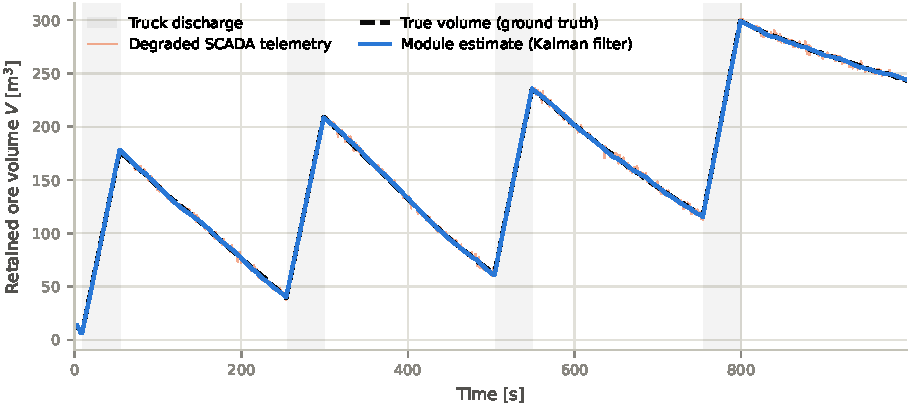
\includegraphics[width=\textwidth]{figuras/fig1_reconstruccion_volumen.pdf}
\caption{Dynamic reconstruction of the retained ore volume in the feed hopper.
Shaded bands indicate truck discharge events.}
\label{fig:reconstr}
\end{figure*}

\subsection{Latent Variable Recovery}

Table~\ref{tab:rate} reports the results on the filling rate, which has no
instrumentation of any kind.

\begin{table}[!t]
\caption{Error Metrics for the Unsensed Filling Rate}
\label{tab:rate}
\centering
\footnotesize
\begin{tabular}{@{}lrrr@{}}
\toprule
\textbf{Metric} & \textbf{Finite diff.} & \textbf{Kalman filter} &
\textbf{Reduction}\\
\midrule
RMSE [m\textsuperscript{3}/s] & 3.6891 & 0.0674 & 98.17\,\%\\
\bottomrule
\end{tabular}
\end{table}

The magnitude of the difference deserves attention. Finite differencing of the
raw signal produces an error of 3.69~m\textsuperscript{3}/s over a physical
quantity whose nominal value is 0.8~m\textsuperscript{3}/s: the procedure does
not return an imprecise estimate, it returns noise with the appearance of a
measurement. Fig.~\ref{fig:latent} contrasts both procedures; note the
difference of scale between panels.

\begin{figure*}[!t]
\centering
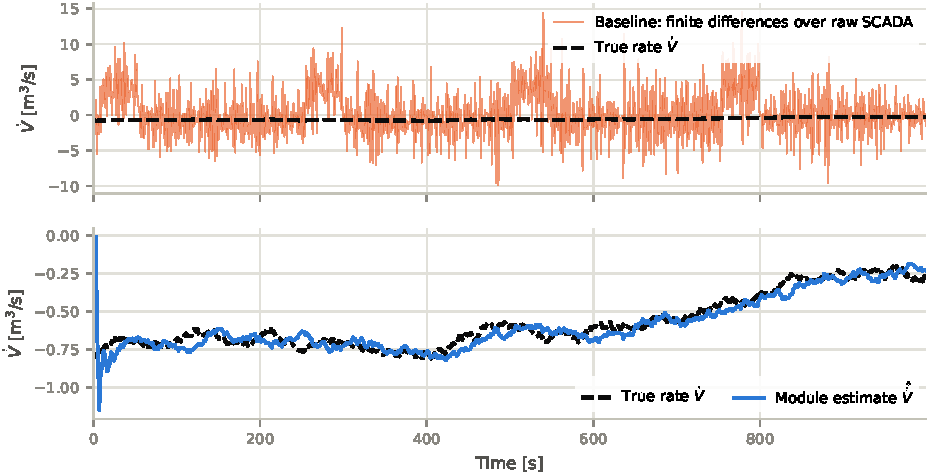
\includegraphics[width=\textwidth]{figuras/fig2_tasa_latente.pdf}
\caption{Recovery of the latent variable. Top: finite-difference baseline over
the raw signal. Bottom: module estimate, at physical scale.}
\label{fig:latent}
\end{figure*}

\subsection{Asymptotic Convergence}

Fig.~\ref{fig:conv} shows the convergence of the error covariance and of the
Kalman gain towards their steady-state values, the behavior predicted by the
Riccati formulation for linear time-invariant systems \cite{simon2006}.
Convergence is reached at around 60~s of operation, with
$K_{1} \rightarrow 0.0993$.

\begin{figure*}[!t]
\centering
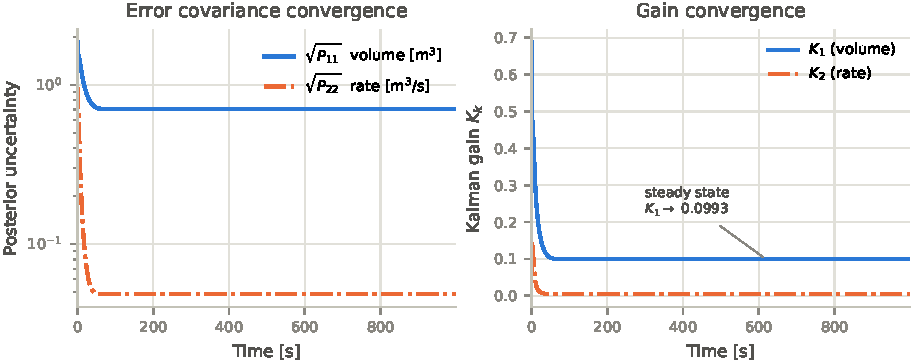
\includegraphics[width=\textwidth]{figuras/fig3_convergencia.pdf}
\caption{Asymptotic convergence of the estimation error covariance and of the
Kalman gain towards steady state.}
\label{fig:conv}
\end{figure*}

\subsection{Statistical Validation}

Table~\ref{tab:stats} reports the inference on the RMSE.

\begin{table}[!t]
\caption{Paired Statistical Inference on Volume RMSE ($M=50$, $\alpha=0.05$)}
\label{tab:stats}
\centering
\footnotesize
\begin{tabular}{@{}lr@{}}
\toprule
\textbf{Statistic} & \textbf{Value}\\
\midrule
Mean RMSE reduction & 1.5106 m\textsuperscript{3}\\
95\,\% confidence interval & $[1.4881,\ 1.5330]$ m\textsuperscript{3}\\
Paired $t$-test (one-sided) & $t(49) = 135.24$; $p = 5.15\times10^{-65}$\\
Effect size (Cohen's $d$) & 19.13\\
Shapiro--Wilk normality & $W = 0.9459$; $p = 0.0233$ (rejected)\\
Wilcoxon signed-rank & $W = 1275.0$; $p = 8.88\times10^{-16}$\\
Decision & $H_{0}$ rejected\\
\bottomrule
\end{tabular}
\end{table}

The normality verification merits comment. The Shapiro--Wilk test
\emph{rejects} normality of the differences ($p = 0.0233 < 0.05$), so a
mechanical application of the $t$-test would be questionable. It is precisely
for this reason that the design incorporated the nonparametric Wilcoxon
contrast, which requires no normality and confirms the conclusion with
$p = 8.88\times10^{-16}$. The agreement of both tests allows $H_{0}$ to be
rejected independently of the parametric assumption. It should be added that
with $M = 50$ observations the central limit theorem grants the $t$-test
considerable robustness to moderate departures from normality, and that the
effect size --- a Cohen's $d$ of 19.13 --- places the result well beyond any
distributional consideration. For the latent state, inference yields
$t(49) = 296.36$ with $p = 1.09\times10^{-81}$ and a 95\,\% confidence interval
of $[3.5971,\ 3.6463]$~m\textsuperscript{3}/s.

\begin{figure*}[!t]
\centering
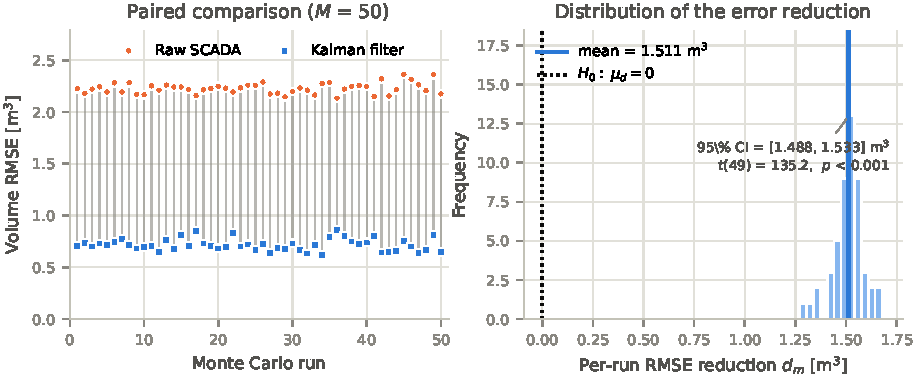
\includegraphics[width=\textwidth]{figuras/fig4_montecarlo.pdf}
\caption{Monte Carlo validation. Left: run-by-run paired comparison. Right:
distribution of the RMSE reduction, with the null hypothesis marked at the
origin.}
\label{fig:mc}
\end{figure*}

\subsection{Sensitivity to Sensor Degradation}

Table~\ref{tab:degrad} and Fig.~\ref{fig:degrad} report the behavior of the
module under increasing levels of true sensor noise.

\begin{table}[!t]
\caption{Module Performance Under Increasing Instrumental Degradation}
\label{tab:degrad}
\centering
\footnotesize
\begin{tabular}{@{}rrrrr@{}}
\toprule
$R$ & $\sigma_{v}$ & MSE SCADA & MSE KF & Reduction\\
{[m\textsuperscript{6}]} & [m\textsuperscript{3}] &
[m\textsuperscript{6}] & [m\textsuperscript{6}] & \\
\midrule
1   & 1.00  & 0.987   & 0.165  & 83.32\,\%\\
5   & 2.24  & 4.937   & 0.527  & 89.33\,\%\\
20  & 4.47  & 19.748  & 1.449  & 92.66\,\%\\
50  & 7.07  & 49.369  & 2.831  & 94.27\,\%\\
100 & 10.00 & 98.738  & 4.707  & 95.23\,\%\\
200 & 14.14 & 197.476 & 7.843  & 96.03\,\%\\
400 & 20.00 & 394.953 & 13.093 & 96.68\,\%\\
\bottomrule
\end{tabular}
\end{table}

Error reduction grows monotonically with the severity of degradation, from
83.32\,\% under benign conditions to 96.68\,\% under extreme degradation. The
contribution of the module therefore does not dilute in hostile environments: it
becomes more pronounced.

\begin{figure*}[!t]
\centering
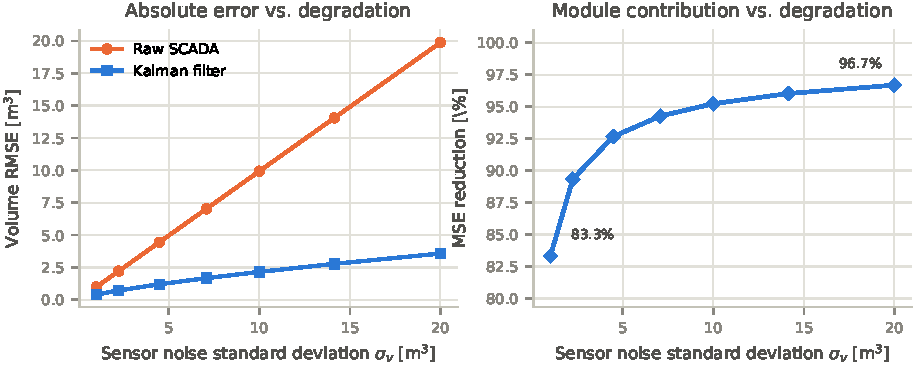
\includegraphics[width=\textwidth]{figuras/fig5_degradacion.pdf}
\caption{Module behavior under increasing instrumental noise. Left: absolute
error of both sources. Right: relative MSE reduction.}
\label{fig:degrad}
\end{figure*}

\subsection{Robustness to Covariance Mismatch}

Fig.~\ref{fig:sens} presents the RMSE grid resulting from deliberately
mistuning the filter covariances with respect to the true physics.

\begin{figure}[!t]
\centering
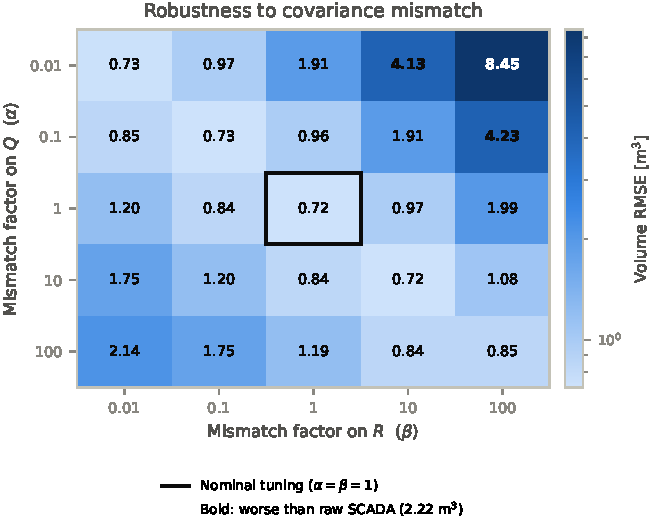
\includegraphics[width=\columnwidth]{figuras/fig6_sensibilidad_QR.pdf}
\caption{Robustness of the module to deliberate mismatch of the $\mathbf{Q}$
and $\mathbf{R}$ covariances. The box marks the nominal tuning.}
\label{fig:sens}
\end{figure}

The result exhibits a marked diagonal structure. Under nominal tuning the RMSE
is 0.721~m\textsuperscript{3}, against 2.224~m\textsuperscript{3} for the raw
telemetry. Along the diagonal, where both covariances are scaled by the same
factor even up to a hundredfold in either direction, performance remains in the
range 0.72--0.85~m\textsuperscript{3}. Severe degradation appears only in the
anti-diagonal corners, with a worst case of 8.45~m\textsuperscript{3}. Of the
twenty-five combinations evaluated, only three are worse than not filtering at
all.

\subsection{Reproducibility}

Two successive independent executions of the experiment produced byte-identical
output files, verified by MD5 checksum over the four generated logs. Exact
reproducibility of the study is therefore a verified fact rather than a
declaration of intent.

% =============================================================================
\section{Discussion}
\label{sec:discussion}

\subsection{Creating Observability Rather Than Denoising}

The most conceptually dense result is not the error reduction on volume but the
reconstruction of the filling rate. On volume, the module improves a signal that
\emph{already exists}: a sensor measures it and the filter reduces its variance.
That is a valuable but incremental contribution. On the filling rate, the module
produces information that \emph{did not exist anywhere in the system}. No
instrument measures it, and the only procedure available to a conventional SCADA
returns noise.

That the module reduces this error by 98.17\,\% means that the analytical layer
is not cleaning data but \emph{creating observability} where instrumentation
provides none. This is the strongest argument for conceiving the estimator as an
architectural component rather than as a preprocessing filter: a preprocessor
improves what it receives, whereas this module delivers to the upper layers a
state variable that was previously unavailable for decision-making.

\subsection{Relation to Prior Work}

The findings give quantitative support to the conceptual distinction of
Sepasgozar \cite{sepasgozar2021}: if the raw telemetry of the filling rate is
essentially noise, a virtual replica fed directly by the SCADA is not
representing the asset but its distortion. The difference between digital shadow
and digital twin ceases to be terminological and acquires a measurable
magnitude.

With respect to mining digital twins, the study aligns with the diagnosis of
Ebad \textit{et al.} \cite{ebad2026} regarding limited industrial validation and
persistent data integration problems, and with the observation of Qu \textit{et
al.} \cite{qu2023} on fragmented adoption. The contribution addresses precisely
the layer both reviews identify as unattended.

With respect to state estimation in mineral processing, the results are
consistent with Apelt \textit{et al.} \cite{apelt2002} in semi-autogenous
grinding and with B\'arzaga-Martell \textit{et al.} \cite{barzaga2025} in copper
heap leaching: non-instrumented internal variables of mining processes are
effectively reconstructible. The difference of the present work is not one of
result but of framing. Those studies formulate estimation as an inferential
measurement or process control instrument; this work formulates it as a
component of a digital twin architecture, with the decoupling, reproducibility
and statistical validation requirements that framing imposes. It is worth noting
that \cite{barzaga2025} employs nonlinear variants while this work deliberately
restricts itself to the linear case: the mass balance of a hopper is genuinely
linear over the operating range considered, and a nonlinear estimator would add
computational cost without precision gain.

\subsection{Practical Implication of the Robustness Finding}

The diagonal structure of the mismatch grid shows that estimator performance is
governed by the \emph{ratio} between covariances rather than by their absolute
values. A calibration error of two orders of magnitude in both matrices
simultaneously degrades the RMSE only from 0.72 to 0.85~m\textsuperscript{3},
whereas the same error applied to a single one raises it to
8.45~m\textsuperscript{3}.

The implication for industrial deployment is direct. The practical difficulty of
tuning a Kalman filter in a plant does not lie in determining the absolute
values of $\mathbf{Q}$ and $\mathbf{R}$, which would require detailed
metrological characterization, but in correctly estimating their proportion,
that is, how much to trust the physical model relative to the sensor. This is a
considerably more accessible task for a process engineer and lowers the adoption
barrier of the module.

\subsection{Limitations}

The principal limitation is that validation is performed on synthetic data
generated by the same model the filter uses. Under that condition the Kalman
filter is optimal by theoretical construction, so the study verifies correct
implementation and quantifies the magnitude of the improvement, but does not
subject the estimator to a genuine model discrepancy. The covariance mismatch
analysis partially mitigates this objection without eliminating it: a real
process may exhibit nonlinearities, correlated or colored noise, and unmodeled
drifts that this design does not reproduce.

A second limitation concerns the scope of the physical model. The implemented
mass balance does not incorporate the real chamber geometry, material size
segregation, or the dependence of extraction rate on instantaneous ore hardness.
Start-up and shutdown transients and blockage events were excluded, which are
precisely the conditions of greatest operational interest.

A third limitation is the absence of validation with real telemetry, a direct
consequence of confidentiality restrictions. This places the work at a
laboratory and simulation technology readiness level, and none of the reported
figures should be interpreted as a prediction of plant performance. Any
deployment on an operating digital twin requires prior on-site piloting and
empirical safety calibration.

% =============================================================================
\section{Conclusion and Future Work}
\label{sec:conclusion}

This paper presented and validated a decoupled analytical software module that
acts as a physical-consistency layer between degraded SCADA telemetry and the
decision layer of a mining digital twin. Over 50 independent Monte Carlo runs,
the module reduced the mean squared error of the retained volume by 89.57\,\%,
a statistically significant reduction robust to the distributional assumption,
and reduced the error on the unsensed filling rate by 98.17\,\%.

The contribution does not lie in the algorithm, established theory since
\cite{kalman1960}, but in three distinct planes: architecturally, the study
formulates stochastic state estimation as a design component of a mining digital
twin rather than as a control instrument or preprocessing stage; empirically, it
provides quantified evidence that the difference between a digital shadow and a
digital twin is measurable, and that the analytical layer can generate
observability where instrumentation provides none; and methodologically, it
delivers a byte-reproducible artifact with traceability logs, verification of
statistical assumptions and parametric robustness analysis, in an area where
effective validation has been reported as a shortcoming.

Four continuation lines are identified. The most immediate is validation with
real telemetry from an operating site, which would allow performance to be
contrasted under genuine model discrepancy and is a necessary condition for any
deployment. The second is extension to nonlinear regimes, incorporating the
start-up, shutdown and blockage conditions excluded here, which would require
migrating towards extended or unscented variants following
\cite{barzaga2025}. The third is adaptive covariance tuning, suggested directly
by the $\mathbf{Q}/\mathbf{R}$ ratio finding: a mechanism adjusting that
proportion online from the innovation sequence would further reduce the
industrial adoption barrier. The fourth is generalization of the module as a
transversal service of the digital twin, applying the same core to the different
subsystems of the asset.

% =============================================================================
\section*{Acknowledgment}

This work was developed within the undergraduate research project of the School
of Informatics, Universidad Andr\'es Bello. The authors thank the reviewers of
the successive project phases for the observations that shaped the statistical
validation design and the dimensional consistency of the reported metrics.

% =============================================================================
\bibliographystyle{IEEEtran}
\bibliography{referencias}

\end{document}
